\documentclass[myclassdoc,debug]{rjparticle}
%use the following command when typesetting your paper:
%\documentclass{rjparticle}
\usepackage{graphicx}

\title{Extensive Study of the Positive and Negative Parity Wobbling States for an Odd-Mass Triaxial Nucleus I} 

\author[1,2,$a$]{R. Poenaru}
\author[2,3,$b$]{A. A. Raduta}

\affil[1]{Doctoral School of Physics, University of Bucharest, Bucharest, Romania\\
\email[a]{robert.poenaru@drd.unibuc.ro} }
\affil[2]{Department of Theoretical Physics - \textit{Horia Hulubei} National Institute for Physics and Nuclear Engineering, M\u{a}gurele-Bucharest, Romania\\
\email[b]{raduta@nipne.ro} (corresponding author)}
\affil[3]{Academy of Romanian Scientists, Bucharest, Romania}

\keywords{Nuclear Structure, Triaxial Nuclei, Wobbling Motion, Parity Symmetry, Signature Partners, Strong Deformation}

\pacs{01.30.-y, 01.30.Ww, 01.30.Xx, 99.00.Bogus}

\hyphenation{rjp-ar-ti-cle}

%%%%%%%%%%%%%%%%%%%%%%%%%%%%%%%%%%%%%%%%%%%%%%%%%%%%%%%%%%%%%%%%%%%%%%%%%%%%%%%
%Please, do not remove the following lines!
%%%%%%%%%%%%%%%%%%%%%%%%%%%%%%%%%%%%%%%%%%%%%%%%%%%%%%%%%%%%%%%%%%%%%%%%%%%%%%%
%\RJPVolume{63}{2018}
%\RJPNumber{1-2}
%\RJPPages{}{}
%\columntitle{Wobbling Nucleus I}
%\date{}
%\dedication{}
%\domaintitle{}
%\keywords{}
%\pacs{01.30.-y, 01.30.Ww, 01.30.Xx, 99.00.Bogus}
%%%%%%%%%%%%%%%%%%%%%%%%%%%%%%%%%%%%%%%%%%%%%%%%%%%%%%%%%%%%%%%%%%%%%%%%%%%%%%%

\begin{document}
%%%%%%%%%%%%%%%%%%%%%%%%%%%%%%%%%%%%%%%%%%%%%%%%%%%%%%%%%%%%%%%%%%%%%%%%%%%%%%%
%Please, remove these lines when typesetting your document!
%%%%%%%%%%%%%%%%%%%%%%%%%%%%%%%%%%%%%%%%%%%%%%%%%%%%%%%%%%%%%%%%%%%%%%%%%%%%%%%
\lstset{%
basicstyle=\small,
language=[AlLaTeX]TeX,
columns=fullflexible,
%keepspaces=true,
showspaces=true,
showstringspaces=false,
keywordstyle=[2]\ttfamily,
identifierstyle=,
texcsstyle=*\ttfamily,
commentstyle=\color{gray},
string=[s]<>,
morestring=[b]',
stringstyle=\emph,
breaklines=true,
deletekeywords={list},
moretexcs={authnote,keywords,pacs},
}
%%%%%%%%%%%%%%%%%%%%%%%%%%%%%%%%%%%%%%%%%%%%%%%%%%%%%%%%%%%%%%%%%%%%%%%%%%%%%%%
\maketitle

\begin{abstract}
A new interpretation of the wobbling structure in $^{163}$Lu is developed. Four wobbling bands are experimentally known in this isotope, where three are wobbling phonon excitations $TSD_{2,3,4}$, and the ground state band, which is $TSD_1$. In this work, a particle-triaxial rotor coupling is considered in a product space of single-particle and collective core states. The single-particle states describe a $j=i_{13/2}$ proton, while the core states characterize the triaxial rotor and are either of positive parity, when the bands $TSD_{1,2,3}$ are concerned or of negative parity for the $TSD_4$ band. There are five free parameters, three moments of inertia, the strength of the particle-core interaction, and the $\gamma$ deformation. A very good description of all 62 experimental states is obtained, with a mean square error of about $80\ \text{keV}$. The newly obtained features evidenced in the present work enrich the knowledge about the wobbling properties of $^{163}$Lu.
\end{abstract}

\section{Introduction}

The experimental observations regarding wobbling motion across the chart of nuclides have been quite rare, even though this kind of collective motion has been theoretically predicted almost 50 years ago by Bohr and Mottelson \cite{bohr1998nuclear} when they were investigating the rotational modes of a triaxial nucleus employing a Triaxial Rotor Model (TRM). Therein, it was shown that for a triaxial rotor, the main rotational motion is around the axis with the largest moment of inertia (MOI), as it is energetically the most favorable. This mode is quantum-mechanically disturbed by the rotation around the other two axes, since rotation around any of the three principal axes of the system are possible, due to the anisotropy between the MOIs (that is $\mathcal{I}_1\neq\mathcal{I}_2\neq\mathcal{I}_3$). The precessional motion of the total angular momentum around the main axis combined with the small oscillations around the other two axes will result in a harmonic-like motion of the deformed nuclear system, with the appearance of rotational bands defined by the wobbling phonon number $n_w=0,1,2,\dots$. Naturally, the description of the energy spectra and electromagnetic transitions between the rotational states of these wobbling nuclei (also known as \emph{wobblers}) are considered to be the main characteristics that are put to the test by a theoretical investigation. The overall agreement between experimental results and the theoretically obtained data serves as an indicator for the quality of the model used to describe the wobbling picture.

This work represents the first part of a two-part series of papers, with the purpose of studying the wobbling phenomenon for odd-mass nuclei with both positive and negative parity states. While the second part will focus on the latest experimental and theoretical progress in the field, together with an analysis of the geometry for a deformed triaxial nucleus (namely, classical trajectories, wobbling stability, and phase transitions), this first paper aims at studying the energy spectrum of $^{163}$Lu in a \emph{semi-classical} approach, where the nuclear states are described through a set of classical equations. By contradistinction with a previous work \cite{raduta2020towards} (which will be hereafter referred to as \texttt{W1}), in here all four wobbling bands are described by the same \emph{core-quasiparticle alignment}, making thus a unified and consistent description of the wobbling motion. A remarking feature for the current research (which will be hereafter referred to as \texttt{W2}) is the introduction of the concept of \emph{Parity Partner Bands} - concerning the states from $TSD_2$ and $TSD_4$ bands -  which will be discussed throughout the paper.


%%%%%%%%%%%%%%%%%%%%% FINISH SECTIONS DESCRIPTION %%%%%%%%%%%%%%%%%%%%
%%%%%%%%%%%%%%%%%%%%%%%%%%%%%%%%%%%%%%%%%%%%%%%%%%%%%%%%%%%%%%%%%%%%%%
The paper is organized as follows. In section \ref{section-reinterpretation}, a discussion on the concepts of Signature Partner Bands and Parity Partner Bands is made, with the introduction of the new \texttt{W2} approach in describing wobbling properties of $^{163}$Lu. A sketch with the required theoretical formalism is done in Section \ref{section-theory}, where the wobbling spectrum for an odd-mass nucleus with both positive and negative parity states is obtained. The numerical results concerning the excitation energies of the four triaxial bands of this isotope are presented in Section \ref{section-results}, where an interpretation of the obtained parameter set is made, together with a comment on the wobbling nature of $^{163}$Lu. Also in Section \ref{section-results}, some other physical quantities specific to triaxial nuclei are discussed. Concluding remarks of the current research are given in Section \ref{section-gata}.
%%%%%%%%%%%%%%%%%%%%%%%%%%%%%%%%%%%%%%%%%%%%%%%%%%%%%%%%%%%%%%%%%%%%%%
%%%%%%%%%%%%%%%%%%%%%%%%%%%%%%%%%%%%%%%%%%%%%%%%%%%%%%%%%%%%%%%%%%%%%%

\section{\texorpdfstring{Re-interpretation of the wobbling bands in $^{163}$Lu}%
                               {Re-interpretation of the wobbling bands structure for 163Lu}}
\label{section-reinterpretation}
Considered the \emph{best wobbler} to date, $^{163}$Lu has a rich wobbling spectrum \cite{odegaard2001evidence,jensen2002evidence}, with no less than four such wobbling bands: one yrast - $TSD_1$, (zero-phonon wobbling number $n_w=0$), and three excited wobbling bands - $TSD_{2,3,4}$ (with their corresponding wobbling phonon numbers $n_w=1,2,3$). The name TSD comes from Triaxial Strongly Deformed bands. The triaxial bands emerge due to the coupling of an odd-$\vec{j}$ nucleon with an even-even triaxial core. Thus, for $^{163}$Lu, it is the intruder $\pi(i_{13/2})$ that couples to the triaxial core \cite{odegaard2001evidence,hamamoto2002wobbling,jensen2002wobbling}, driving the nuclear system up to large deformation, and stabilizing the deformed structure. Indeed, a triaxial shape with deformation parameters \cite{bohr1998nuclear} $(\beta_2,\gamma)\approx(0.38,+20^\circ)$ is assumed to be in agreement with the observed data, based on calculations using the Ultimate Cranker Code \cite{bengtsson1990high} for the potential energy surface (PES).

In terms of the experimental evidence which should be pointing out the wobbling nature of $^{163}$Lu, the large transition quadrupole moment $Q_t \approx 10\ b$ \cite{gorgen2004quadrupole}, the predominantly $E2$ character of the transitions linking adjacent bands ($I\to I-1$), a large $E2/M1$ mixing ratio $\delta>1$ for the transitions linking the yrare ($n_w=1$) and yrast ($n_w=0$) bands are all clear fingerprints of wobbling nature. Another quantity that indicates strong deformation with wobbling character is the relative rigid rotor energy, and for this isotope, calculations show that all four bands have similar behavior with respect to this value (see Figs. 3 and 4 from Ref. \cite{hagemann2005triaxiality}). For a set of results concerning these quantities (both theoretical and experimental), see Refs. \cite{raduta2017semiclassical,raduta2020new}, and the references cited therein. 

\subsection{Signature Partner Bands + Parity Partner Bands}
\label{subsection:w2}

In \texttt{W1} it was shown that through a re-normalization of the four wobbling bands belonging to $^{163}$Lu, all wobbling properties can be successfully described within a semi-classical approach based on the Particle-Rotor-Model (PRM) \cite{bohr1998nuclear,hamamoto2002wobbling,frauendorf2014transverse,tanabe2006algebraic,wen2015wobbling}. Indeed, the bands $TSD_1$ and $TSD_2$ were considered as ground-state \emph{Signature Partner Pairs}, with the former (latter) being the favored (un-favored) signature partner. The two bands are formed by coupling an $i_{13/2}$ valence proton with a triaxial core of even spins $R_1=0,2,4,\dots$ in the case of $TSD_1$ and odd spins $R_2=1,3,5,\dots$ for $TSD_2$. The third band ($TSD_3$) is the one-wobbling-phonon excitation built on top of $TSD_2$.  However, in order to account for the negative parity states belonging to $TSD_4$ (a ground-state band with zero-wobbling-phonon number), a different quasi-particle alignment was proposed throughout the calculations, more precisely the $h_{9/2}$ proton (with negative parity) that couples to a core of odd-spin states $R_2=1,3,5,\dots$. This results in having two sets of deformation parameters that describe the wobbling properties of the nucleus, namely one set for the bands $TSD_{1,2,3}$, and a second one for $TSD_4$. By comparison, the new \texttt{W2} formalism will consider a unique single-particle (the $j=13/2$ proton from $i$-th orbital, denoted throughout the paper with $j_1$), but with a slight adjustment for the triaxial core. Namely the newly adopted coupling scheme is defined as follows: 
\begin{enumerate}
    \item Coupling $C'_1$: the odd $j_1$ proton aligns with the core of even-integer spin sequence $R_1=0^+,2^+,4^+,\dots$, with a parity of the $R_1$ core that is positive $\pi(R_1)=+1$.
    \item Coupling $C'_2$: the odd $j_1$ proton aligns with the core of even-integer spin sequence $R_2^+=1^+,3^+,5^+,\dots$, with a parity of the $R_2^+$ core that is positive $\pi(R_2^+)=+1$.
    \item Coupling $C'_3$: the odd $j_1$ proton aligns with the core with an odd-integer spin sequence $R_2^-=1^-,3^-,5^-,\dots$, which has negative parity $\pi(R_2^-)=-1$.
\end{enumerate}

From the three schemes defined above, it is clear that $C'_1$ corresponds to the yrast $TSD_1$, $C'_2$ to the ground state $TSD_2$, and finally $C'_3$ to the ground state $TSD_4$. Obviously, the odd valence nucleon $j_1$ has a positive parity $\pi_{j_1}=+1$. There has not been attributed a coupling scheme for $TSD_3$, since this band remains as the one-wobbling phonon excitation which is built on top of $TSD_2$.

The last step in searching for a unified coupling scheme in $^{163}$Lu is to establish a possible relationship between the four bands. As per the calculations involved in \texttt{W1}, it was proven that signature is a good quantum number and indeed, a sign that $TSD_1$ and $TSD_2$ are signature partners emerged. Their overall similar properties and spin difference enforce this argument. Furthermore, in this new \texttt{W2} approach, the difference in parity between the $TSD_2$ and $TSD_4$ but the same angular momentum sequence of their corresponding triaxial core $R_2^+$ and $R_2^-$ strongly suggest that the two bands are \emph{Parity Partner Bands}: two rotational sequences with energy states characterized by opposite parity, increasing energy that follows a trend $\propto I(I+1)$, and a spin difference $\Delta I=2$ between states belonging to the same band. Calculations that will show that parity is indeed a good quantum number for the triaxial rotor + odd-particle system will be provided in the following sections. For what it is worth mentioning is that the concept of parity partners between $TSD_2$ and $TSD_4$ emerge from the idea that a stable deformed structure is achieved from a single quasiparticle which \emph{moves inside} a quadrupole mean-field generated by a triaxial even-even core. However, there is a splitting in two different cases of coupling mechanisms, namely $C'_2$/$C'_3$ depending on the alignment of the high-$j$-shell particle with a core of positive/negative parity.

Similar structures with alternating positive-negative parity bands have been also reported in other nuclei such as $^{40}$Ca \cite{torilov2004spectroscopy}, or some heavier isotopes like $^{218}$Fr \cite{debray2000alternating}. A unified description of states with positive and negative parity in odd-mass nuclei was made over the last decade \cite{radutaa2009csm,raduta2011simultaneous}, although therein, a quadrupole-octupole term was introduced within the particle-core Hamiltonian to describe this feature.

\section{Theoretical Formalism}
\label{section-theory}

In this section, a description of the framework used for obtaining the wobbling spectrum of $^{163}$Lu is made. As stated, the system is described with a similar Hamiltonian used in \texttt{W1}, namely the Hamiltonian for the triaxial PRM: 
\begin{align}
    H=H_\text{core}+H_\text{s.p.}\ .
    \label{prm-hamiltonian}
\end{align}

The Hamiltonian from Eq. \ref{prm-hamiltonian} describes a system in which an odd $j$ particle interacts with a triaxial core, i.e., the odd nucleon is moving in a quadrupole deformed mean-field that is generated by the core. As such, the first term in the Hamiltonian $H_\text{core}$ corresponds to the motion of a triaxial core, while the second term $H_\text{s.p.}$ represents the single-particle potential characterizing the valence proton. For the first term of $H$:
\begin{align}
    H_\text{core}=\sum_{i=1,2,3}\frac{1}{2\mathcal{I}_i}(I_i-j_i)^2\ ,
    \label{core-hamiltonian}
\end{align}
where the core angular momentum is $\vec{R}=\vec{I}-\vec{j}$ and the terms $\mathcal{I}_i$ represent the moments of inertia for a triaxial ellipsoid, along the principal axes. These three moments of inertia will be considered as free parameters in the present calculations, but, compared to the work \texttt{W1}, a unique set of MOIs will be attributed to the four bands. Because of this, there is no option for their nature (i.e., rigid or hydrodynamic).

Second term of Eq. \ref{prm-hamiltonian} is derived from the well-known Nilsson potential \cite{meyer1975collective,wang2008description}:
\begin{align}
    H_\text{s.p.}=\frac{V}{j(j+1)}\left[\cos\gamma(3j_3^2-\vec{j}^2)-\sqrt{3}\sin\gamma(j_1^2-j_2^2)\right]+\epsilon_j\ .
    \label{single-particle-hamiltonian}
\end{align}

This term describes the motion of an odd particle with angular momentum $j$ in a mean-field generated by a triaxial core, with a potential strength $V$ characterized by the quadrupole deformation ($V\propto\beta_2)$. The single-particle potential strength $V$ will be considered as the fourth free parameter within the calculations and its value will dictate the coupling of the $j$ particle with all four TSD bands. The term $\epsilon_j$ from Eq. \ref{single-particle-hamiltonian} represents the single-particle energy that corresponds to the odd $j$ proton from the $i$-orbital. One should not mix up the $j_1$ proton notation used throughout the paper with the components of the single-particle angular momentum from  Eq. \ref{single-particle-hamiltonian}. Regarding the triaxial deformation $\gamma$ which enters in Eq. \ref{single-particle-hamiltonian}, its value will be considered as another free parameter of the current problem.

From Eqs. \ref{core-hamiltonian} and \ref{single-particle-hamiltonian}, the free parameter set can be obtained, hereafter denoted by $\mathcal{P}$. It comprises three moments of inertia, the single-particle potential strength, and the triaxial deformation. As such, $\mathcal{P}$ can be written as:
\begin{align}
    \mathcal{P}=\left[\mathcal{I}_1,\mathcal{I}_2,\mathcal{I}_3,V,\gamma\right]\ .
    \label{parameter-set}
\end{align}

Finding the energy spectrum for $^{163}$Lu within \texttt{W2} is equivalent with finding the eigenvalues of $H$ given in Eq. \ref{prm-hamiltonian}. In a similar approach as in \texttt{W1}, the eigenvalues of interest are obtained on the base of a semi-classical approach. Thus, the first step is to perform a de-quantization procedure on $H$ through a Time Dependent Variational Principle Equation (TDVE) \cite{raduta2007semiclassical,budaca2018tilted,raduta2017semiclassical,raduta2020new}:
\begin{align}
    \delta\int_0^t\bra{\Psi_{IjM}}H-i\frac{\partial}{\partial t'}\ket{\Psi_{IjM}}dt'=0\ .
    \label{tdve}
\end{align}

The rest of the calculations are not given explicitly here, due to space limitations and also due to the similarities between the de-quantization procedure involved in \texttt{W1} and \texttt{W2}, however they can be followed according to Refs. \cite{raduta2018wobbling,raduta2020approach,raduta2020towards}. It is essential to point out that by adopting a de-quantization procedure via TDVE, a set of classical equations of motion describing the nucleus can be obtained. Under some restrictions for the MOIs (namely the three moments must be $\mathcal{I}_1>\mathcal{I}_2>\mathcal{I}_3$), the solutions of these equations can be real and positive (hereafter denoted with $\Omega_1^I$ and $\Omega_2^I$, where $\Omega_1^I<\Omega_2^I$) defined for $j_1=i_{13/2}$, given by:
\begin{align}
    \Omega_{1,2}^I=\sqrt{\frac{1}{2}\left(-B\mp(B^2-4C)^{1/2}\right)}\ .
    \label{wobbling-frequencies}
\end{align}

These two solutions (with $B$ and $C$ terms given in \texttt{W1}) are interpreted as \emph{wobbling frequencies} associated with the motion of the core, and the motion of the odd-particle, respectively. As such, each wobbling frequency has an corresponding wobbling-phonon number $\Omega_1^I \to n_{w_1}$ and $\Omega_2^I \to n_{w_2}$.


Now  the analytical expressions for the four TSD bands in $^{163}$Lu are readily obtained:
\begin{align}
    E_\text{TSD1}^I&=\epsilon_j+\mathcal{H}_\text{min}^{(I,j)}+\mathcal{F}_{00}^I\ ,\ I=13/2,17/2,21/2\dots \nonumber \\
    E_\text{TSD2}^I&=\epsilon_j^1+\mathcal{H}_\text{min}^{(I,j)}+\mathcal{F}_{00}^I\ ,\ I=27/2,31/2,35/2\dots \nonumber \\
    E_\text{TSD3}^I&=\epsilon_j+\mathcal{H}_\text{min}^{(I-1,j)}+\mathcal{F}_{10}^{I-1}\ ,\ I=33/2,37/2,41/2\dots \nonumber \\
    E_\text{TSD4}^I&=\epsilon_j^2+\mathcal{H}_\text{min}^{(I,j)}+\mathcal{F}_{00}^I\ ,\ I=47/2,51/2,55/2\dots\ ,
    \label{wobbling_energies}
\end{align}
where $\mathcal{F}_{n_{w_1}n_{w_2}}^I$ is a function of the wobbling frequencies:
\begin{align}
    \mathcal{F}_{n_{w_1}n_{w_2}}^I=\Omega_1^I\left(n_{w_1}+\frac{1}{2}\right)+\Omega_2^I\left(n_{w_2}+\frac{1}{2}\right)\ ,
    \label{f-term}
\end{align}
and $\mathcal{H}_\text{min}^{(I,j)}$ is the classical energy evaluated in its minimal point. For the present case, its analytical expression is given by the following equation:
\begin{align}
\mathcal{H}_\text{min}^{(I,j)}=(A_2+A_3)\frac{I+j}{2}+A_1(I-j)^2-V\frac{2j-1}{j+1}\sin\left(\gamma+\frac{\pi}{6}\right)\ .
    \label{hmin:equation}
\end{align}

A few aspects regarding the energy spectrum defined in Eq. \ref{wobbling_energies} are worth mentioning. To each band, there is a specific energy $\epsilon_j$ associated with the single-particle state. In this case, the odd-proton $j_1=i_{13/2}$ is the one that couples to the triaxial core. However, for the bands $TSD_2$ and $TSD_4$, a different re-normalization of $\epsilon_j$ is considered, since $TSD_2$ is the unfavored signature partner of $TSD_1$, and $TSD_4$ is the negative parity partner of $TSD_2$ within the band structure. These quantities will shift the overall energy states belonging to the two bands, each by a different amount. As a result, both $\epsilon_j^1$ and $\epsilon_j^2$ will be adjusted throughout the numerical calculations such that the energy spectrum is best reproduced. Another aspect concerns the band $TSD_3$; since this is the only excited wobbling band within the family, its configuration is built on top of $TSD_2$, with the action of a single phonon ($n_{w_1}=1$) operator. Consequently, an energy state $I$ belonging to $TSD_3$ is obtained from a state $I-1$ from $TSD_2$. In Table \ref{energy-states-tabular}, the rest of the wobbling phonon numbers are mentioned, with the parity, signature, and coupling scheme for each band in particular.

\begin{table}
\caption{The wobbling phonon numbers, parities, signatures, and coupling schemes assigned to each triaxial band in $^{163}$Lu, within the \texttt{W2} model. The three coupling schemes were defined in Section \ref{subsection:w2}.}
\centering
\begin{tabular}{llllll}
\hline
Band & $n_{w_1}$ & $n_{w_2}$ & $\pi$ & $\alpha$ & Coupling scheme\\
\hline
\hline
   $TSD_1$  &   0        &    0       & +1      &    +1/2      &   $C'_1$              \\
   $TSD_2$  &     0      &      0     &   +1    &  -1/2        &   $C'_2$              \\
   $TSD_3$  &   1        &      0     &     +1  &     +1/2    &  Built on top of $TSD_2$                \\
   $TSD_4$  &    0       &      0     &      -1 &   -1/2       &    $C'_3$    \\       
   \hline
\end{tabular}
\label{energy-states-tabular}
\end{table}

\subsection{Parity quantum number for the wave-function}

In \texttt{W1} it was shown that signature emerges from the calculations on the total wave function as a good quantum number for this triaxial system. This is why in \cite{raduta2020approach} the bands $TSD_1$ and $TSD_2$ appeared as Signature Partner Bands (SPB). In \texttt{W2}, such property still stands.

Since the backbone of the current work started from the need for a single odd-particle that couples to a triaxial core in $^{163}$Lu, one has to look at the band $TSD_4$ (which was interpreted as having a different nucleon: $j_2$ with $j=9/2$ from the $h$-orbital), and see if its differentiating properties can be linked to \emph{main group} of bands (namely $TSD_{1,2,3}$). Indeed, from the experimental measurements regarding spin and parity assignment \cite{jensen2004coexisting}, it turns out that the parity of the rotational states is negative. Therefore, forensic analysis on this quantum property should be considered as the necessary ingredient in a unified description of all four bands.

 The parity operator is defined as a product of the complex conjugation operation and a rotation of angle $\pi$ around the 2-axis: $P=e^{-i\pi\hat{I}_2}C$. The total parity operator is the product of an operator corresponding to the core and one corresponding to the single-particle:
\begin{align}
    \mathcal{P}_T=P_\text{core}P_\text{s.p.}\ .
    \label{parity-operator}
\end{align}

Acting with the total parity operator defined above, on the trial function $\Psi$ associated , the following result is obtained:
\begin{align}
    \mathcal{P}_T\Psi(r,\varphi;t,\psi)=\Psi(r,\varphi+\pi;t,\psi+\pi)\overset{\mathrm{not.}}{=}\ \bar{\Psi}.
    \label{parity-action}
\end{align}

The classical energy function $\mathcal{H}$ has an invariance property at changing the angles with $\pi$:
\begin{align}
    \mathcal{H}(r,\varphi;t,\psi)=\mathcal{H}(r,\varphi+\pi;t,\psi+\pi)\ .
    \label{classical-energy-invariance}
\end{align}

From Eqs. \ref{parity-action} and \ref{classical-energy-invariance}, it can be concluded that the wave-function describing the triaxial system $\Psi$ and its image through $\mathcal{P}_T$ , $\bar{\Psi}$,  are two linearly dependent functions which differ only by a multiplicative constant $p$, with $|p|=1$. Thus, $p$ can either be -1 or +1, such that:
\begin{align}
    % \Psi(r,\varphi+\pi;t,\psi+\pi)=\pm\Psi(r,\varphi;t,\psi)\ .
    \bar{\Psi}=\pm\Psi(r,\varphi;t,\psi)\ .
\end{align}

The above result concludes the parity analysis for the wave function, showing that the triaxial rotor admits eigenfunctions of negative parity. Therefore, a single wave function characterized by the coupling of a triaxial core to the odd proton $i_{13/2}$ is describing both positive parity states ($\in TSD_{1,2,3}$) as well as negative parity states ($\in TSD_4$). This analysis, together with the fact that $TSD_2$ and $TSD_4$ have the same angular momentum sequences (although $TSD_2$ has more low-lying states than $TSD_4$) suggests the fact that these two bands behave as Parity Partners.


\section{Numerical results}
\label{section-results}

As a first step, the results concerning the excited spectrum of the four TSD bands will be presented. Regarding the wobbling spectrum of $^{163}$Lu, its analytical formulation was given in Eq. \ref{wobbling_energies}. As mentioned, those energies are parametrized in terms of $\mathcal{P}$, which is the set of free parameters to be determined. Indeed, one can find $\mathcal{P}$ by minimizing the $\chi^2$ function:
\begin{align}
    \chi^2=\frac{1}{N_T}\sum_{i}\frac{(E^{(i)}_\text{exp}-E^{(i)}_\text{th})^2}{E^{(i)}_\text{exp}}\ ,
    \label{chi-square}
\end{align}
where $N_T$ represents the total number of states. Table \ref{4-band-information} contains the number of states within each band, with the spin sequences for the core ($\vec{R}$), the spin sequences for the coupled system (that is the total angular momentum $\vec{I})$, and the coupling schemes specific to \texttt{W2} formalism that is used in the current calculations. 

\begin{table}
\caption{The number of energy states $n_s$ within each wobbling band, the a.m. of the proton $\vec{j}$, the core's a.m. $\vec{R}$, the nucleus' a.m. $\vec{I}$, and the corresponding coupling scheme that was established according to the \texttt{W2} model. The single-particle is the $j_1=(i_{13/2})$ proton.}
    \centering
  \begin{tabular}{llllll}
  \hline
  Band & $n_s$ & $\vec{j}$ & $\vec{R}$ - Sequence & $\vec{I}$ - Sequence & Coupling  \\
  \hline
  \hline
     $TSD_1$ &       21      &   $j_1$  &        $R_1=0^+,2^+,4^+,\dots$         &   $13/2,17/2,21/2,\dots$    & $C'_1$     \\
     $TSD_2$ &        17     &   $j_1$   &       $R_2^+=1^+,3^+,5^+,\dots$             &      $27/2,31/2,35/2,\dots$                &      $C'_2$           \\
     $TSD_3$ &      14       &    $j_1$  &           1-phonon exc.         & $33/2,37/2,41/2,\dots$                &       1-phonon exc.           \\
     $TSD_4$ &       11      &   $j_1$   &    $R_2^-=1^-,3^-,5^-,\dots$                &               $47/2,51/2,55/2,\dots$         &      $C'_3$          \\
     \hline
\end{tabular}
    \label{4-band-information}
\end{table}

The resulting values for $\mathcal{P}$ are given  in Table \ref{parameter_set}. This \texttt{W2} method contrasts the approach in \texttt{W1}, where a second minimization process was needed separately for $TSD_4$. The root mean square error provided by the obtained parameter set $\mathcal{P}$ has a value of $E_\text{rms}\approx 79\ \text{keV}$. This result is much better than the one obtained with previous formalism \texttt{W1} where an $E_\text{rms}\approx240\ \text{keV}$ was obtained \cite{raduta2020approach}. This is the first semi-classical formalism in the literature that achieves agreement with the experimental data with less than $100\ \text{keV}$ for the entire wobbling spectrum of $^{163}$Lu. It is worth mentioning that the fitting procedure was done not for the absolute wobbling energies $E_\text{TSDk}^I\ ,\ k=1,2,3,4$, but for the \emph{excitation energies} which are relative to the hand-head $I^{\pi}=13/2^+$ from the $TSD_1$. Comparison between the theoretical values obtained within the current formalism and the experimental data is shown in Figs. \ref{energies-tsd12} and \ref{energies-tsd34}. For the sake of completeness, the wobbling frequencies which enter in the expression of the $\mathcal{F}_{n_{w_1}n_{w_2}}^I$ given by Eq. \ref{f-term} are graphically represented as functions of total angular momentum $I$ in Fig. \ref{hydro-mois}, for the fixed parameter set. It is remarkable the fact that the wobbling frequency $\Omega_2^I$ is much larger than its partner, suggesting the fact the coupling effects caused by the highly aligned proton have a stronger influence in achieving a wobbling character for $^{163}$Lu, which is in line with the characteristics of a particle-rotor coupling. Another feature of these wobbling frequencies is their linear behavior with respect to the nuclear spin.

\begin{table}
\caption{The parameter set $\mathcal{P}$ that was determined by a fitting procedure of the excitation energies for $^{163}$Lu.}
    \centering
  \begin{tabular}{lllll}
  \hline
$\mathcal{I}_1$ [$\hbar^2$/\text{MeV}] & $\mathcal{I}_2$ [$\hbar^2$/\text{MeV}]& $\mathcal{I}_3$ [$\hbar^2$/\text{MeV}] & $\gamma$ [deg. ] & $V$ [\text{MeV}] \\
\hline
\hline
72              & 15              & 7               & 22       & 2.1\\
\hline
\end{tabular}
    \label{parameter_set}
\end{table}

Concerning the single-particle energies from Eq. \ref{wobbling_energies}, namely $\epsilon_j^1$ and $\epsilon_j^2$ that emerge from the un-favored signature of $TSD_2$ and negative parity of $TSD_4$, respectively, they induce a correction for the mean-field with the quantities $\epsilon_j^1-\epsilon_j=0.3\ \text{MeV}$ and $\epsilon_j^2-\epsilon_j=0.6\ \text{MeV}$. Note that since the energy state $I_{13/2}\in TSD_1$ (the band-head of $TSD_1$) was subtracted from all bands, the single-particle energies for band 2 and 4 are adjusted accordingly.

The quantity $\epsilon_j^1-e_j$ is added to the second band due to the core, and such a splitting is caused by the fact that two distinct TDVE procedures were performed for the two partner bands $TSD_{1,2}$. The total signature splitting for the band-head and the terminus states of $TSD_2$ are $E_{TSD2}^{27/2}-E_{TSD2}^{25/2}=0.492\ \text{MeV}$ and $E_{TSD2}^{91/2}-E_{TSD2}^{89/2}=0.936\ \text{MeV}$ which agrees with the estimate made by Jensen et. al. in \cite{jensen2002wobbling}. Although the signature splitting can be determined microscopically by using a deformed single-particle basis amended with a cranking constraint, for the present case it is obtained by applying the TDVE for each spin state and the correction corresponding to the single-particle energies (that is $\epsilon_j^1$).

\begin{figure}
\centering
\begin{minipage}{.5\textwidth}
  \centering
  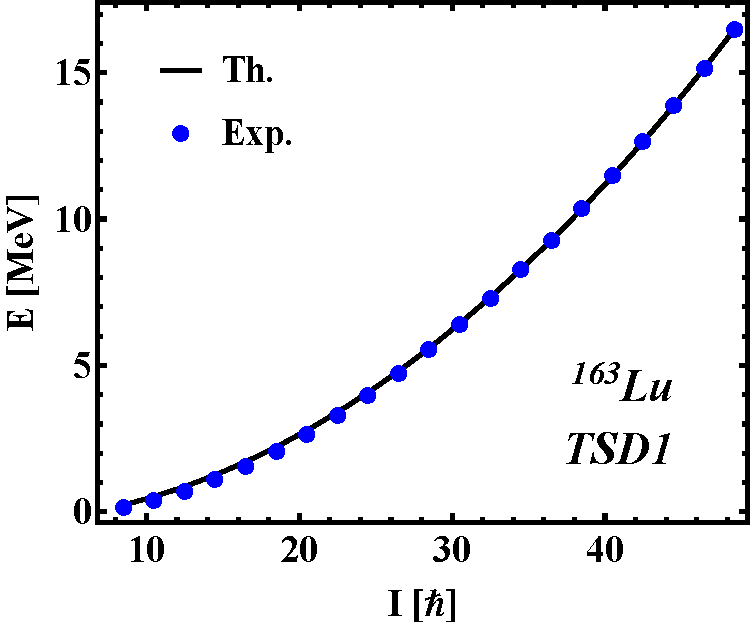
\includegraphics[scale=0.45]{figs/DoubleShift_TSD1.pdf}
\end{minipage}%
\begin{minipage}{.5\textwidth}
  \centering
 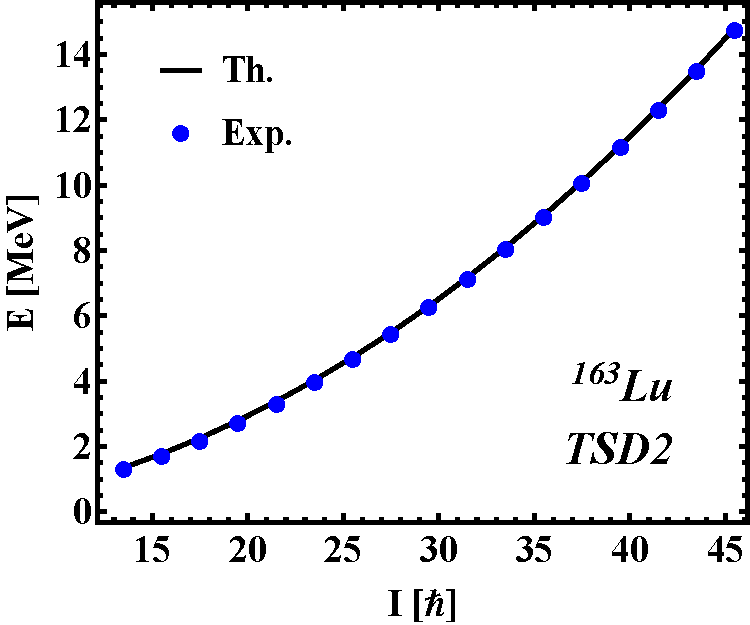
\includegraphics[scale=0.45]{figs/DoubleShift_TSD2.pdf}
\end{minipage}
\caption{Comparison between theoretical and experimental excitation energies for the first two wobbling bands in $^{163}$Lu within the \texttt{W2} model. The theoretical results are obtained with the parameters listed in Table \ref{parameter_set}. Experimental data is taken from \cite{reich2010nuclear}.}
\label{energies-tsd12}
\end{figure}

\begin{figure}
\centering
\begin{minipage}{.5\textwidth}
  \centering
  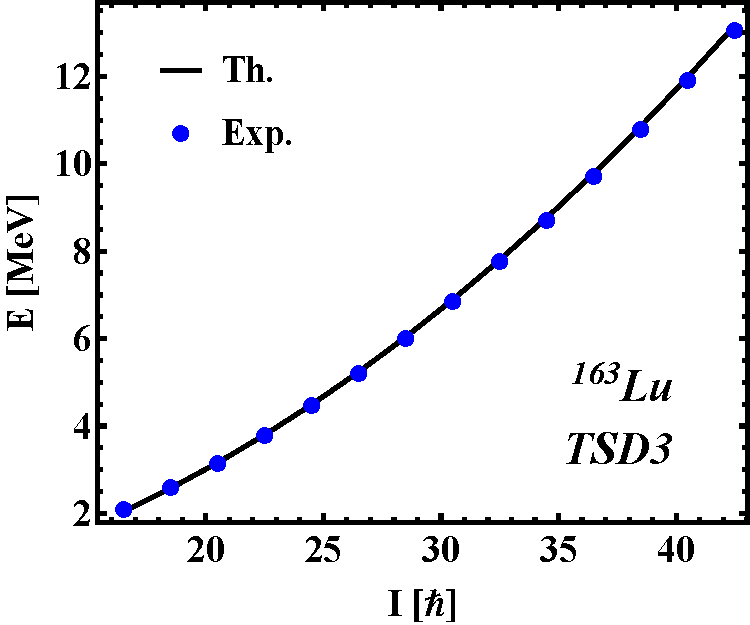
\includegraphics[scale=0.45]{figs/DoubleShift_TSD3.pdf}
\end{minipage}%
\begin{minipage}{.5\textwidth}
  \centering
 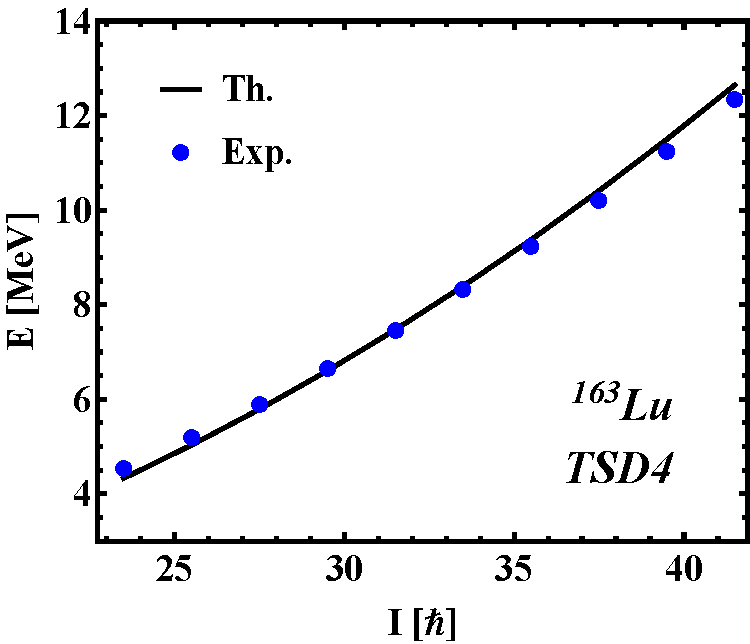
\includegraphics[scale=0.45]{figs/DoubleShift_TSD4.pdf}
\end{minipage}
\caption{Comparison between theoretical and experimental excitation energies for third and fourth wobbling bands in $^{163}$Lu within the \texttt{W2} model. The theoretical results are obtained with the parameters listed in Table \ref{parameter_set}. Experimental data is taken from \cite{reich2010nuclear}.}
    \label{energies-tsd34}
\end{figure}

Another noteworthy aspect of the current formalism is the fact that the difference $\delta_{42}=E_\text{TSD4}^I-E_\text{TSD2}^I$ for all the states has an almost constant value $\delta_{42}\approx0.3\ \text{MeV}$. This suggests that the states of the same angular momentum from $TSD_2$ and $TSD_4$ bands might emerge through the parity projection of a sole wave function that does not have reflection symmetry. In the present case, this is caused by the fact that the wobbling frequency is parity-independent. Interestingly, the action of the parity operator on any rotational state within the angular momentum space will lead to the change of the angular momentum vector from $\vec{I}$ to $-\vec{I}$. Due to this reason, the parity operator commutes with the initial Hamiltonian, and the eigenfunctions of $H$ are characterized by either positive or negative parity (with states of different parities being degenerate). However, one can lift this degeneracy by using an additional linear in the expression $H$. Since in Eq. \ref{prm-hamiltonian} such a linear term is missing, an \emph{ad-hoc} correction of the mean-field with the amount $0.6\ \text{MeV}$ for the states in $TSD_4$ is necessary. As a result, the added shift simulates the breaking of parity symmetry. In contrast to this approach, when using a microscopic formalism, one starts with a single-particle basis generated by a mean-field without space reflection symmetry, followed by the calculation of the many-body wave-functions (being admixtures of both positive and negative parities). Restoration of the parity symmetry is achieved by selecting from all the wave-functions only the components with a definite parity (projecting the good parity), leading to a doublet structure of positive and negative parity states in the spectrum of $H$. Consequently, the bands $TSD_2$ and $TSD_4$ behave as a pair of parity partners, as defined in \cite{chasman1980incipient,raduta2006description,raduta2006simultaneous}.

% \subsection{Interpretation of the parameter set $\mathcal{P}$}
\subsection{\texorpdfstring{Interpretation of the parameter set $\mathcal{P}$}%
                               {Interpretation of the parameter set P}}\label{results:interpret}

Performing the fitting procedure for the excitation energies of $^{163}$Lu will result in the moments of inertia $\mathcal{I}_k$ that are given in Table \ref{parameter_set}, together with the single-particle potential strength $V$, and triaxiality parameter $\gamma$. Interpretation of their numerical values is mandatory in order to check whether the current formalism is valid or not.

Regarding the moments of inertia, it is clear that the axis of rotation for the ellipsoid is the 1-axis, as the largest MOI is $\mathcal{I}_1$. The MOI ordering is $\mathcal{I}_1>\mathcal{I}_2>\mathcal{I}_3$, and compared with the results of the previous work \texttt{W1}, the current 1-axis MOI is bigger than both $\mathcal{I}_1^\text{TSD1,2,3}=63.2\ \hbar^2/\text{MeV}$ and $\mathcal{I}_1^\text{TSD4}=67\ \hbar^2/\text{MeV}$ (data taken from Table 1 in Ref. \cite{raduta2020towards}). This is expected, since here, the $TSD_4$ band is obtained by the coupling of a particle from a higher $j$-shell, driving the system to an even larger deformation. One must remember that these are the \emph{effective} MOIs of the entire system, that is the triaxial-rotor + odd-particle. No spin dependence has been inferred for the MOIs, so a possible change in the MOIs ordering with the increase in spin $I$ cannot be studied within the current description. Furthermore, this formalism does not contain microscopic terms, so no presumptions on what causes the obtained MOI ordering can be stated. Although, by working with a quadrupole deformed mean-field, the moments of inertia of the triaxial core should be indeed consistent with the hydrodynamic model, which for the sake of completeness are shown in Fig. \ref{hydro-mois}.

\begin{figure}
\centering
\begin{minipage}{.5\textwidth}
  \centering
  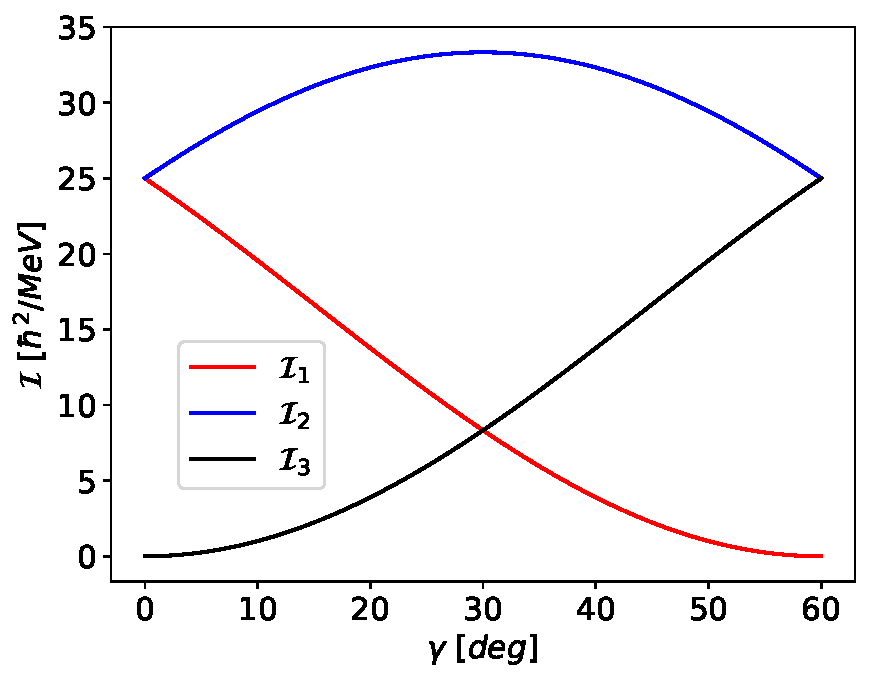
\includegraphics[scale=0.44]{figs/hydro_mois.pdf}
\end{minipage}%
\begin{minipage}{.5\textwidth}
  \centering
 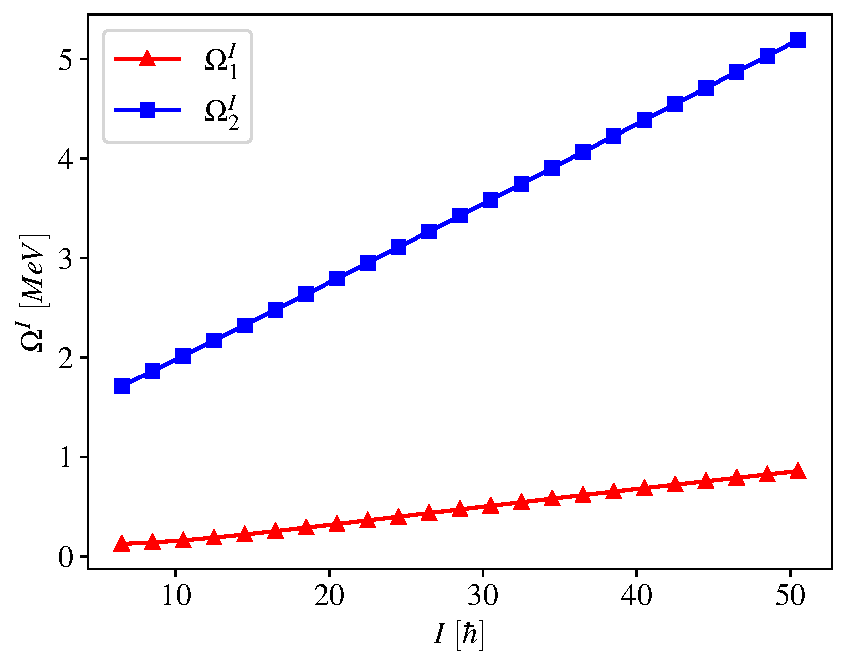
\includegraphics[scale=0.44]{figs/wobbling-frequencies.pdf}
\end{minipage}
\caption{Left-side: The hydrodynamic moments of inertia \cite{tanabe2006algebraic} as function of the triaxiality parameter $\gamma$, for the positive interval $\gamma\in[0^{\circ},60^{\circ}]$, evaluated for a scale factor $\mathcal{I}_0=25\ \text{MeV}^{-1}$. Right-side: The wobbling frequencies defined in Eq. \ref{wobbling-frequencies} as function of total angular momentum, evaluated with the parameter set $\mathcal{P}$ which was obtained through the fitting procedure.}
    \label{hydro-mois}
\end{figure}

% Concerning the triaxiality parameter $\gamma$, it has a positive value $\gamma=22^\circ$. This is consistent with the microscopic descriptions based on cranking mechanism for the potential energy surface (PES) of $^{163}$Lu. In fact, the agreement is quite good with the predicted deformed minima of $(\beta_2,\gamma)\approx(0.38,20^\circ)$ \cite{jensen2002wobbling,jensen2004coexisting}. Comparing the current \texttt{W2} model with already existing descriptions which take $\gamma$ to be fixed a-priori throughout the calculations (e.g., \cite{tanabe2006algebraic,tanabe2017stability}), here $\gamma$ is obtained through the fitting process in a self-consistent manner. Moreover, its value is slightly larger than the one obtained in \texttt{W1} formalism ($\gamma=17^\circ$). This might be due to the larger ratios $\mathcal{I}_1/\mathcal{I}_{2,3}$, which in the present case they appear to be bigger ($\mathcal{I}_1/\mathcal{I}_{2}\approx4.8$ for \texttt{W2}, compared to $\approx3.2$ in the previous approach \text{W1}).
Concerning the triaxiality parameter $\gamma$, a value of $\gamma=22^\circ$ was obtained via the fitting procedure. The agreement is quite good with the predicted deformed minima of $(\beta_2,\gamma)\approx(0.38,20^\circ)$ \cite{jensen2002wobbling,jensen2004coexisting}. By comparison, other formalisms which aim at describing the wobbling properties of $^{163}$Lu take the value of $\gamma$ to be fixed a-priori thrughout the calculations \cite{tanabe2006algebraic,tanabe2017stability}). Remarkable the fact that the obtained value is slightly larger than the one from \texttt{W1} ($\gamma=17^\circ$). This might be due to the larger ratios $\mathcal{I}_1/\mathcal{I}_{2,3}$, which in the present case they appear to be bigger ($\mathcal{I}_1/\mathcal{I}_{2}\approx4.8$ for \texttt{W2}, compared to $\approx3.2$ in the previous approach \text{W1}).

Lastly, the single-particle potential strength has a value of $V=2.1\ \text{MeV}$. In \texttt{W1}, this parameter was $V^{\text{TSD1,2,3}}=3.1\ \text{MeV}$ and $V^\text{TSD4}=0.7\ \text{MeV}$. An explanation for its decrease in the present case might be due to the upward shift in the energy caused by the un-favored partner, or due to the energetic shift of the parity partner, indicating a quenching effect on the quadrupole deformation of the triaxial system due to either the signature splitting ($TSD_{1-2}$) or the parity symmetry breaking ($TSD_{2-4}$). Nevertheless, the obtained value seems to be consistent with the previous calculations, the current value of $V$ being close to the average value of the two $V$'s from $\texttt{W1}$. Other interpretations \cite{tanabe2017stability} that were developed using a similar single-particle potential term in the Hamiltonian adopted values of around $V=1.6\ \text{MeV}$, however, that was for an isotope with smaller quadrupole deformation $\beta_2=0.18$. Interesting research using a single-$j$ shell model which was aimed at obtaining a realistic expression for the deformation parameter has been performed in \cite{shou2009coupling}. Therein, results for the potential strength of odd-$A$ nuclei with similar mass, but different quasiparticle configurations were numerically obtained. Concluding this subsection, the obtained values of $\mathcal{P}$ seem to not only describe the wobbling spectrum of $^{163}$Lu very well (see results in Figs. \ref{energies-tsd12} and \ref{energies-tsd34}), but they are also consistent with the previous formalism \texttt{W1}, or even with other interpretations from the literature. 

% \subsection{Comment on the wobbling nature of $^{163}$Lu}
\subsection{\texorpdfstring{Comment on the wobbling nature of $^{163}$Lu}%
                               {Comment on the wobbling nature of 163Lu}}\label{wobbling-comment}

According to Frauendorf et al. \cite{frauendorf2014transverse}, the wobbling character of a nucleus is given by the coupling of the odd particle which aligns its angular momentum parallel or perpendicular to the axis with the largest MOI (marking two different wobbling regimes called \emph{longitudinal} LW and \emph{transverse} TW, respectively). Also from \cite{frauendorf2014transverse}, it is considered that based on the wobbling regime, a particular behavior of the wobbling energy $E_\text{wob}$ as defined in Eq. \ref{wobbling-energy-relative} will be observed: the energy $E_\text{wob}$ increases with spin for LW and it decreases for TW. Experimentally, $E_\text{wob}$ is obtained by subtracting the energy state of the first excited wobbling band (the one-wobbling-phonon band, denoted by index $1$) from the average of its adjacent energies that belong to the yrast partner (denoted by index $0$). In the present calculations, the first excited state is $TSD_3$, with its yrast partner being the band $TSD_2$. Following this procedure, both the experimental wobbling energies, as well as the theoretical ones were calculated according to Eq. \ref{wobbling-energy-relative}. The obtained results are plotted in Fig. \ref{wobbling-energies_th_exp}.
\begin{align}
    E_\text{wob}(I)=E_{1}(I)-\left(\frac{E_0(I+1)+E_0(I-1)}{2}\right)\ ,
    \label{wobbling-energy-relative}
\end{align}

\begin{figure}
    \centering
    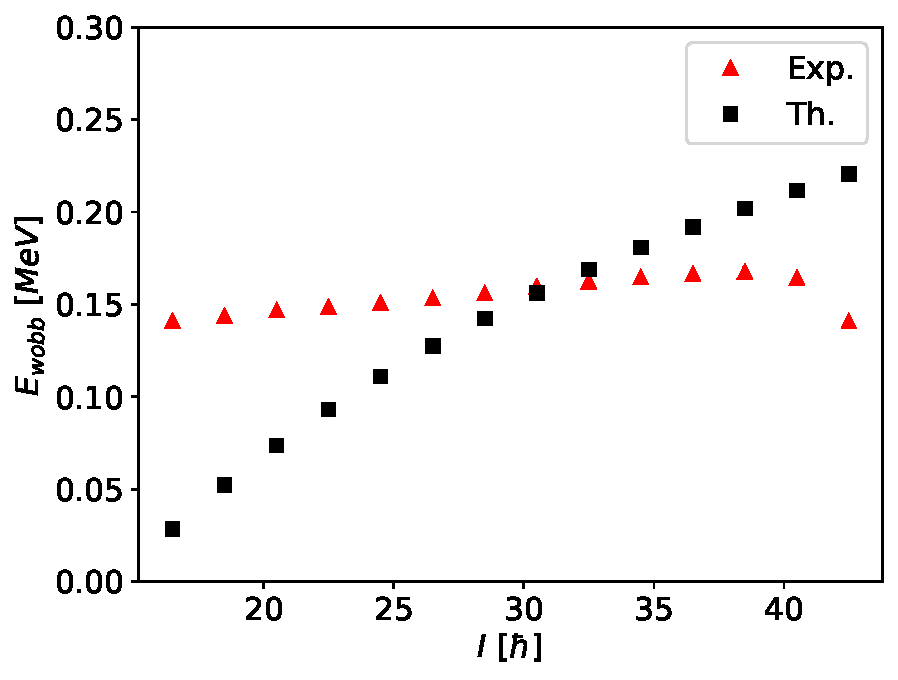
\includegraphics[scale=0.4]{figs/wobbling_energy_ThExp.pdf}
    \caption{The wobbling energies for $^{163}$Lu given as $E_\text{wob}=E_1(I)-\frac{1}{2}(E_0(I+1)+E_0(I-1))$. According to the current $\texttt{W2}$ formalism, the sets of energies $E_1$ belong to $TSD_3$, while $E_0$ correspond to $TSD_2$. Experimental data is taken from \cite{reich2010nuclear}. Theoretical values were calculated with the parameter set $\mathcal{P}$.}
    \label{wobbling-energies_th_exp}
\end{figure}

From the behavior of $E_\text{wob}$ from Fig. \ref{wobbling-energies_th_exp}, it can be seen that the theoretical wobbling spectrum is an increasing function of angular momentum $I$, suggesting that $^{163}$Lu would have an LW character. This contrasts other interpretations for $^{163}$Lu on which the wobbling energy decreases with respect to increasing angular momentum $I$  \cite{frauendorf2014transverse,frauendorf2018comment, tanabe2018reply}. However, within those formalisms, the wobbling energies are obtained with $TSD_2$ and $TSD_1$.

Analyzing the experimental data points from Fig. \ref{wobbling-energies_th_exp}, a slight increase with spin can also be observed, suggesting as well that the coupling scheme in $^{163}$Lu achieves an LW character. Indeed, from the lower limit of around $11/2\ \hbar$ and up to a spin of about $39/2\ \hbar$, the energy is increasing, then it starts to decrease once the spin reaches a critical value $I_\text{cr}\geq39/2\ \hbar$. The identification of a \emph{critical} region in which a nucleus with mass $A\approx160$ could change its wobbling regime (e.g., from LW to TW) is another remarking feature of the current formalism, as this is the first time when such behavior is identified for this mass region. The increasing behavior of the theoretical data also appears to be quenched in the high-spin limit, indicating that once the nucleus reaches high spins, a change in the wobbling regime might emerge.

In a recent study for the wobbling motion in $^{183}$Au made by Nandi et al. \cite{nandi2020first}, the two observed wobbling bands are based on different alignments: the $\pi(i_{13/2})$ nucleon (for the so-called \emph{positive parity band}) and the $\pi(h_{9/2})$ nucleon (for the \emph{negative-parity} band) coupled to a triaxial rotor, respectively. The remarking aspect of this research is that within a PRM model amended with the HFA (harmonic frozen alignment \cite{frauendorf2014transverse}) approximation, it is implied that the configuration of both bands have a transverse (TW) character. However, the wobbling energies $E_\text{wob}$ in these bands have different behavior concerning the increase of angular momentum. Namely, $E_\text{wob}$ increases (decreases) with spin for the positive (negative) parity configurations (see Figs. 3 and 5 from \cite{nandi2020first}). This indicates that an increasing/decreasing behavior for $E_\text{wob}$ is not enough evidence for asserting a wobbling character on a triaxial nucleus (at least, not without some strong constraints on the coupling scheme between the core and the odd particle).

Concluding this comment on the wobbling nature for $^{163}$Lu, if the behavior of the wobbling energies with respect to increasing angular momentum is the sole player in determining the wobbling character of a nucleus, then one could argue that indeed, based on the current results, $^{163}$Lu behaves as a longitudinal wobbler. On the other hand, considering the newly obtained results discussed in the previous paragraph, the evidence is not enough for making a clear assumption on which type of wobbling motion occurs.

\subsection{Other physical quantities}\label{subsection:routhians}

It is instructive to make a quantitative analysis on other relevant properties which are of interest for deformed nuclei. The comparison between theory and experiment of these values can be considered as another test on the correctness of the \texttt{W2} formalism. As such, the rotational/angular frequency $\hbar\omega$ as a function of total angular momentum $I$ is studied for all four bands. One can consider this quantity as the frequency of the electromagnetic radiation emitted by a rotating triaxial nucleus, in correspondence to classical electrodynamics. Any modifications to the nucleonic motion are directly \emph{embedded} in $\hbar\omega$, since the inertial forces depend on the angular frequency. For rotational bands with $\Delta I=2$, the experimental rotational frequency at given angular momentum $I$ is $\hbar\omega_I=\frac{1}{2}\left(E_I-E_{I-2}\right)$. The theoretical results are compared with the experimental ones in Fig. \ref{hrot_plots}. A good overall agreement across all spectrum can be observed with a range for $\hbar\omega$ between $0.2-0.6$ MeV. The linear increase of $\hbar\omega$ suggests that with increasing spin, each transition from a state $I$ to a state $I-2$ will be more energetic.
\begin{figure}
\centering
\begin{minipage}{.5\textwidth}
  \centering
  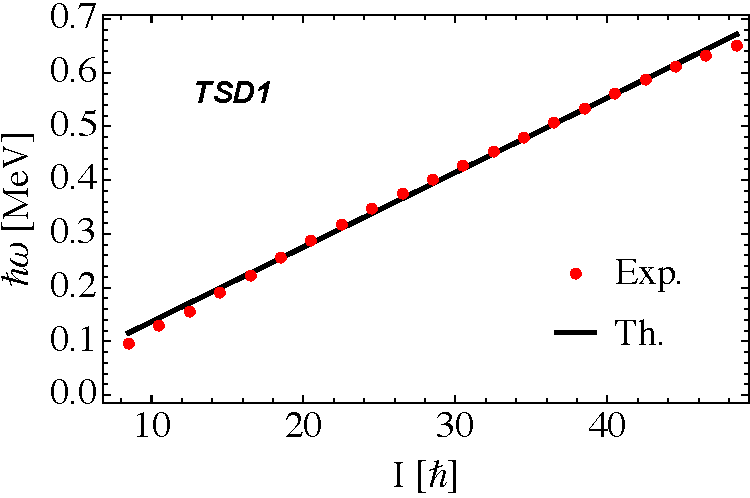
\includegraphics[scale=0.44]{figs/hrot_tsd1.pdf}
  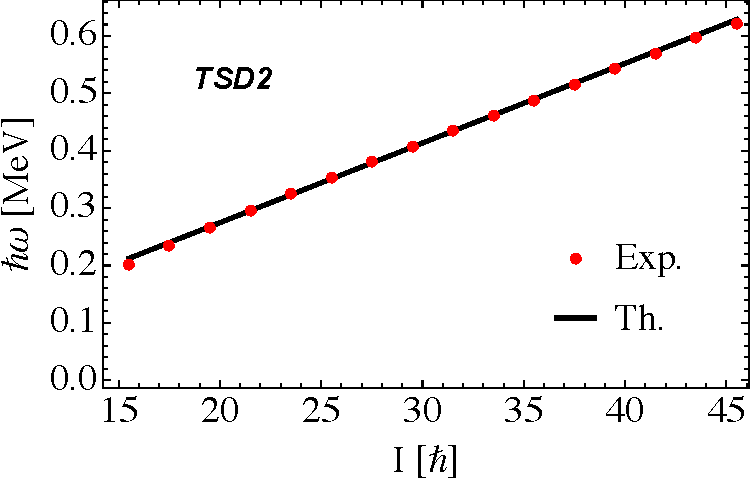
\includegraphics[scale=0.44]{figs/hrot_tsd2.pdf}
\end{minipage}%
\begin{minipage}{.5\textwidth}
  \centering
 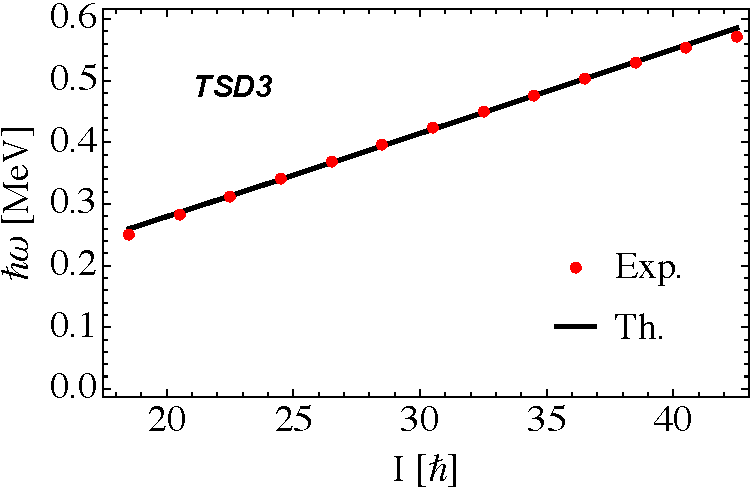
\includegraphics[scale=0.44]{figs/hrot_tsd3.pdf}
 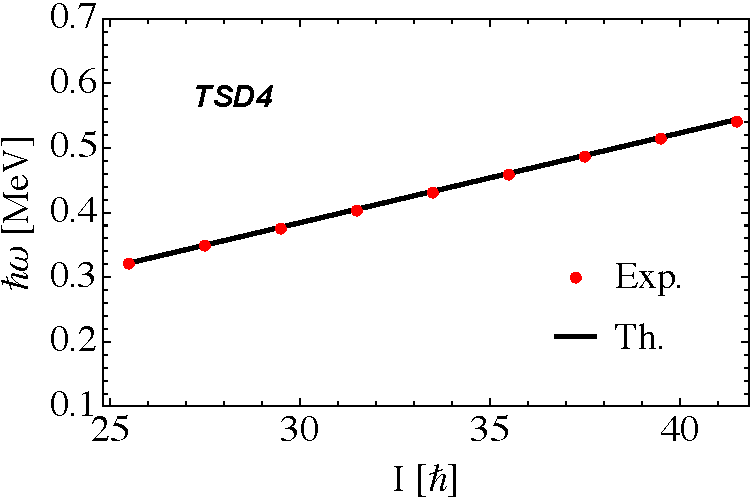
\includegraphics[scale=0.44]{figs/hrot_tsd4.pdf}
\end{minipage}
\caption{The rotational frequencies of$^{163}$Lu, calculated for the obtained parameter set $\mathcal{P}$.}
    \label{hrot_plots}
\end{figure}

Another important quantity worth discussing is the intrinsic energy of the nucleus, evaluated in the rotating frame (also known as Routhian). The importance of such quantity has been discussed in detail by Bengtsson \cite{bengtsson1979quasiparticle}. Taken at a given rotational frequency, the bands above the yrast line may be interpreted as the particle-hole or quasiparticle excitations, and since the Routhians are built from the rotational frequencies, the study of their evolution with respect to the rotational frequency might give an insight into the underlying particle-core couplings. For an odd-mass nucleus, with $\Delta I=2$ rotational bands, the Routhians can be determined via the expression of the rotational frequency as such:
\begin{align}
    E'(I,\hbar\omega)=\frac{1}{2}\left(E_{I}+E_{I-2}\right)-\mathcal{J}\cdot\hbar\omega\ ,
\end{align}
where $\mathcal{J}$ is approximated as $I-\frac{1}{2}$. Since the rotational frequency can be determined from the excitation energy of two consecutive spins within a $TSD$ band, a graphical representation of $E'$ as a function of $I$ is more convenient from a computational standpoint (although it is equivalent to a representation as a function of $\hbar\omega$). These results can be seen in Fig. \ref{routhians_plot}, and the theoretical values which are obtained from the fitting parameters seem to agree with the experimental data quite well, especially the bands $TSD_{1,2,3}$. The fourth triaxial band has a less pronounced decrease in magnitude with respect to spin, marking a drawback of the ad-hoc correction which was made for the negative parity states, namely that it cannot account for the rapid downward slope of $E'$. From the quite similar behavior of all four curves, one can conclude that indeed, $^{163}$Lu has the same particle alignment in all of the four triaxial bands.
\begin{figure}
  \centering
  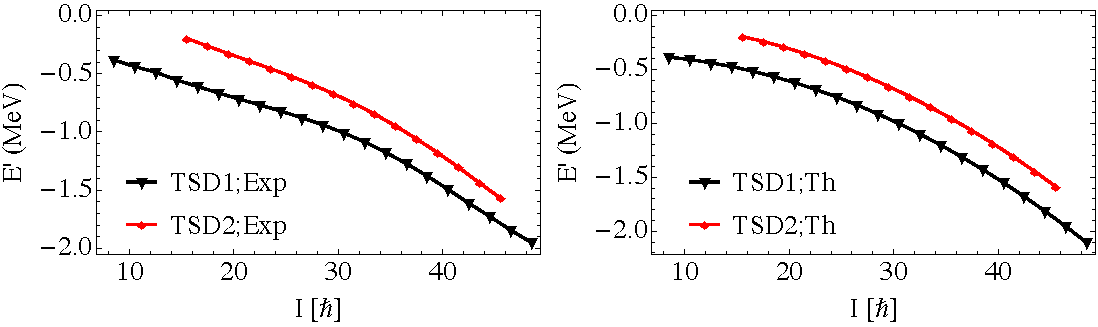
\includegraphics[scale=0.65]{figs/routhians12.pdf}
 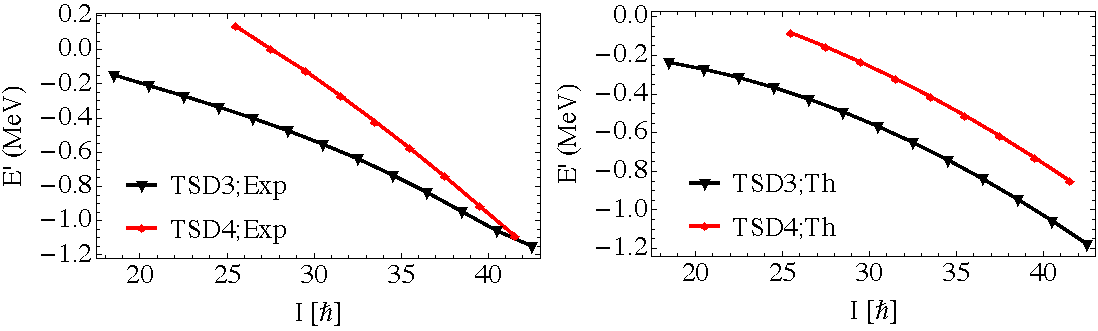
\includegraphics[scale=0.65]{figs/routhians34.pdf}
\caption{The Routhian $E'$ as a function of angular momentum for $^{163}$Lu. The representation is completely equivalent to the one as a function of rotational frequency $\hbar\omega$. A rigid rotor reference $31.7(\hbar\omega)^2\ \text{MeV}^{-1}$ has been subtracted from $E'$.}
    \label{routhians_plot}
\end{figure}

\section{Conclusions \& Outlook}
\label{section-gata}
The objective of the current paper was to extend a previous model that describes the $^{163}$Lu using a re-interpretation of its four wobbling bands. The previous model (denoted here by \texttt{W1}) introduced the concept of signature partners between the bands $TSD_1$ and $TSD_2$. In \texttt{W1}, the $i_{13/2}$ proton was involved in the particle-rotor-coupling for the first three bands, while another proton with negative parity (i.e., $\pi(h_{9/2})$) for band $TSD_4$. Here all bands are described by the coupling of a unique single-particle ($i_{13/2}$ with positive parity $\pi_{j}=+1$) to the core spin-states of positive parity for $TSD_{1,2,3}$ and core spins-states of negative parity for $TSD_4$. The coupling schemes for the wobbling bands within \texttt{W2} were denoted throughout the paper by $C'_1, C'_2, C'_3$ (see discussion in Section \ref{subsection:w2}). From the quantal Hamiltonian specific to a Particle Rotor Model (given by Eq. \ref{prm-hamiltonian}), by applying a Time-Dependent Variational Principle (TDVE) as in Eq. \ref{tdve} with the trial function carefully chosen so that it allows a mixture of both positive and negative parity states, a set of analytical expressions for the excitation energies of each band were obtained (defined in Eq. \ref{wobbling_energies}).

From the theoretical formalism for the excitation energies of $^{163}$Lu, a set of free parameters emerged, containing the three moments of inertia, the single-particle potential strength $V$, and the triaxiality parameter $\gamma$. They were obtained through a fitting procedure which was done for all four bands, unlike the previous \texttt{W1} approach. An impressive agreement between the existing theoretical and experimental data concerning the wobbling spectrum of this isotope was achieved, with an r.m.s. of about $79\ \text{keV}$. The numerical values for the obtained parameters were interpreted in Section \ref{results:interpret}, and indeed, the obtained values are consistent with other formalisms from the literature. A discussion on the wobbling character of $^{163}$Lu is also made in Section \ref{wobbling-comment}, where the critical spin-region for this isotope was identified. Lastly, quantities like rotational frequencies and intrinsic energies in the rotating frame were calculated and compared with the experimental data, showing an overall good agreement between the two sets of data (see Section \ref{subsection:routhians}).
\begin{acknowledgement}
This work was supported by UEFISCU, through the project \textbf{PCE-16/2021}.
\end{acknowledgement}

\begin{thebibliography}{99}

\bibitem{bohr1998nuclear}
Aage~Niels Bohr and Ben~R Mottelson.
\newblock{\em Nuclear Structure (In 2 Volumes)}.

\bibitem{raduta2020towards}
AA~Raduta, R~Poenaru, and CM~Raduta.
\newblock{\em Journal of Physics G: Nuclear and Particle Physics},
  47(2):025101, 2020.

\bibitem{odegaard2001evidence}
SW~{\O}deg{\aa}rd, GB~Hagemann, DR~Jensen, M~Bergstr{\"o}m, B~Herskind,
  G~Sletten, S~T{\"o}rm{\"a}nen, JN~Wilson, PO~Tj{\o}m, I~Hamamoto, et~al.
\newblock{\em Physical review letters}, 86(26):5866, 2001.

\bibitem{jensen2002evidence}
DR~Jensen, GB~Hagemann, I~Hamamoto, SW~{\O}deg{\aa}rd, B~Herskind, G~Sletten,
  JN~Wilson, K~Spohr, H~H{\"u}bel, P~Bringel, et~al.
\newblock{\em Physical review letters}, 89(14):142503, 2002.

\bibitem{jensen2002wobbling}
D~Ringk{\o}bing Jensen, GB~Hagemann, I~Hamamoto, SW~{\O}deg{\aa}rd,
  M~Bergstr{\"o}m, B~Herskind, G~Sletten, S~T{\"o}rm{\"a}nen, JN~Wilson,
  PO~Tj{\o}m, et~al.
\newblock{\em Nuclear Physics A}, 703(1-2):3--44, 2002.

\bibitem{nandi2020first}
S~Nandi, G~Mukherjee, QB~Chen, S~Frauendorf, R~Banik, Soumik Bhattacharya,
  Shabir Dar, S~Bhattacharyya, C~Bhattacharya, S~Chatterjee, et~al.
\newblock{\em Physical Review Letters}, 125(13):132501, 2020.

\bibitem{frauendorf2014transverse}
S~Frauendorf and F~D{\"o}nau.
\newblock{\em Physical Review C}, 89(1):014322, 2014.

\bibitem{hamamoto2002wobbling}
Ikuko Hamamoto.
\newblock{\em Physical Review C}, 65(4):044305, 2002.

\bibitem{tanabe2006algebraic}
Kosai Tanabe and Kazuko Sugawara-Tanabe.
\newblock{\em Physical Review C}, 73(3):034305, 2006.

\bibitem{wen2015wobbling}
Shi Wen-Xian and Chen Qi-Bo.
\newblock{\em Chinese Physics C}, 39(5):054105, 2015.

\bibitem{raduta2017semiclassical}
AA~Raduta, R~Poenaru, and L~Gr Ixaru.
\newblock{\em Physical Review C}, 96(5):054320, 2017.

\bibitem{raduta2020new}
AA~Raduta, CM~Raduta, and R~Poenaru.
\newblock{\em Journal of Physics G: Nuclear and Particle Physics},
  48(1):015106, 2020.

\bibitem{raduta2007semiclassical}
AA~Raduta, R~Budaca, and CM~Raduta.
\newblock{\em Physical Review C}, 76(6):064309, 2007.

\bibitem{raduta2018wobbling}
AA~Raduta, R~Poenaru, and Al~H Raduta.
\newblock{\em Journal of Physics G: Nuclear and Particle Physics},
  45(10):105104, 2018.

\bibitem{budaca2018tilted}
R~Budaca.
\newblock{\em Physical Review C}, 97(2):024302, 2018.

\bibitem{raduta2020approach}
AA~Raduta, R~Poenaru, and CM~Raduta.
\newblock{\em Physical Review C}, 101(1):014302, 2020.

\bibitem{bengtsson1990high}
Tord Bengtsson.
\newblock{\em Nuclear Physics A}, 512(1):124--148, 1990.

\bibitem{gorgen2004quadrupole}
A~G{\"o}rgen, RM~Clark, M~Cromaz, P~Fallon, GB~Hagemann, H~H{\"u}bel, IY~Lee,
  AO~Macchiavelli, G~Sletten, D~Ward, et~al.
\newblock{\em Physical Review C}, 69(3):031301, 2004.

\bibitem{hagemann2005triaxiality}
GB~Hagemann.
\newblock{\em Acta Physica Polonica B}, 36(4):1043, 2005.

\bibitem{jensen2004coexisting}
DR~Jensen, GB~Hagemann, I~Hamamoto, B~Herskind, G~Sletten, JN~Wilson,
  SW~{\O}deg{\aa}rd, K~Spohr, H~H{\"u}bel, P~Bringel, et~al.
\newblock{\em The European Physical Journal A-Hadrons and Nuclei},
  19(2):173--185, 2004.

\bibitem{tanabe2017stability}
Kosai Tanabe and Kazuko Sugawara-Tanabe.
\newblock{\em Physical Review C}, 95(6):064315, 2017.

\bibitem{frauendorf2018comment}
S~Frauendorf.
\newblock{\em Physical Review C}, 97(6):069801, 2018.

\bibitem{tanabe2018reply}
Kosai Tanabe and Kazuko Sugawara-Tanabe.
\newblock{\em Physical Review C}, 97(6):069802, 2018.

\bibitem{torilov2004spectroscopy}
S~Torilov, S~Thummerer, W~Von~Oertzen, Tz~Kokalova, G~De~Angelis, HG~Bohlen,
  A~Tumino, M~Axiotis, E~Farnea, N~Marginean, et~al.
\newblock{\em The European Physical Journal A-Hadrons and Nuclei},
  19(3):307--317, 2004.

\bibitem{debray2000alternating}
ME~Debray, MA~Cardona, D~Hojman, AJ~Kreiner, M~Davidson, J~Davidson, H~Somacal,
  G~Levinton, DR~Napoli, S~Lenzi, et~al.
\newblock{\em Physical Review C}, 62(2):024304, 2000.

\bibitem{radutaa2009csm}
AA~Radutaa and CM~Radutab.
\newblock{\em arXiv preprint arXiv:0903.0076}, 2009.

\bibitem{raduta2011simultaneous}
AA~Raduta and CM~Raduta.
\newblock{\em Annals of the University of Craiova, Physics}, 21(1):28--53,
  2011.

\bibitem{meyer1975collective}
J~Meyer-ter Vehn.
\newblock{\em Nuclear Physics A}, 249(1):111--140, 1975.

\bibitem{wang2008description}
SY~Wang, SQ~Zhang, B~Qi, J~Peng, JM~Yao, J~Meng, et~al.
\newblock{\em Physical Review C}, 77(3):034314, 2008.

\bibitem{reich2010nuclear}
CW~Reich and Balraj Singh.
\newblock{\em Nuclear Data Sheets}, 111(5):1211--1469, 2010.

\bibitem{chasman1980incipient}
RR~Chasman.
\newblock{\em Physics Letters B}, 96(1-2):7--10, 1980.

\bibitem{raduta2006description}
AA~Raduta, CM~Raduta, and Amand Faessler.
\newblock{\em Physics Letters B}, 635(2-3):80--84, 2006.

\bibitem{raduta2006simultaneous}
AA~Raduta, Al~H Raduta, and CM~Raduta.
\newblock{\em Physical Review C}, 74(4):044312, 2006.

\bibitem{shou2009coupling}
Wang Shou-Yu, Qi~Bin, and Zhang Shuang-Quan.
\newblock{\em Chinese Physics Letters}, 26(5):052102, 2009.

\bibitem{bengtsson1979quasiparticle}
R~Bengtsson and S~Frauendorf.
\newblock {\em Nuclear Physics A}, 327(1):139--171, 1979.
\end{thebibliography}

\end{document}